\section{Comparison}
\label{section:comparison}

\par In this section, a global comparison between Octave and Ngspice results will be made. 

\par As requested we were able to compute the passband frequency in simulation analysis using the measure funtion and the central frequency in the theoretical analysis as already explained. Moreover, the POP-AMP model is far more complex in Ngspice than in Octave.The different calculation methods lead to the difference between both methods. The calculated and simulated impedances have the same issues. However, our results were fairly satisfying.


 \begin{table}[h]
\parbox{.45\linewidth}{
  \centering
  \begin{tabular}{|l|r|}
    \hline    
    {\bf Calculus} & {\bf Value} \\ \hline
    V Gain&36.3869\\ \hline
Bandwidth&1.27868E+06\\ \hline
Lower Cut Off Freq& 53.0031\\ \hline

  \end{tabular}
  \caption{Central frequency [Hz] and respective gain [dB]. (Ngspice)}} 
\parbox{.45\linewidth}{
 \centering
  \begin{tabular}{|l|r|}
    \hline    
    {\bf Name} & {\bf Value} \\ \hline
    \input{../mat/wo_freq_gain_TAB}
  \end{tabular}
  \caption{Central frequency [Hz] and respective gain [dB]. (Octave)}}
\end{table}



\begin{figure}[ht]
\centering
\parbox{.49\linewidth}{
  \centering
  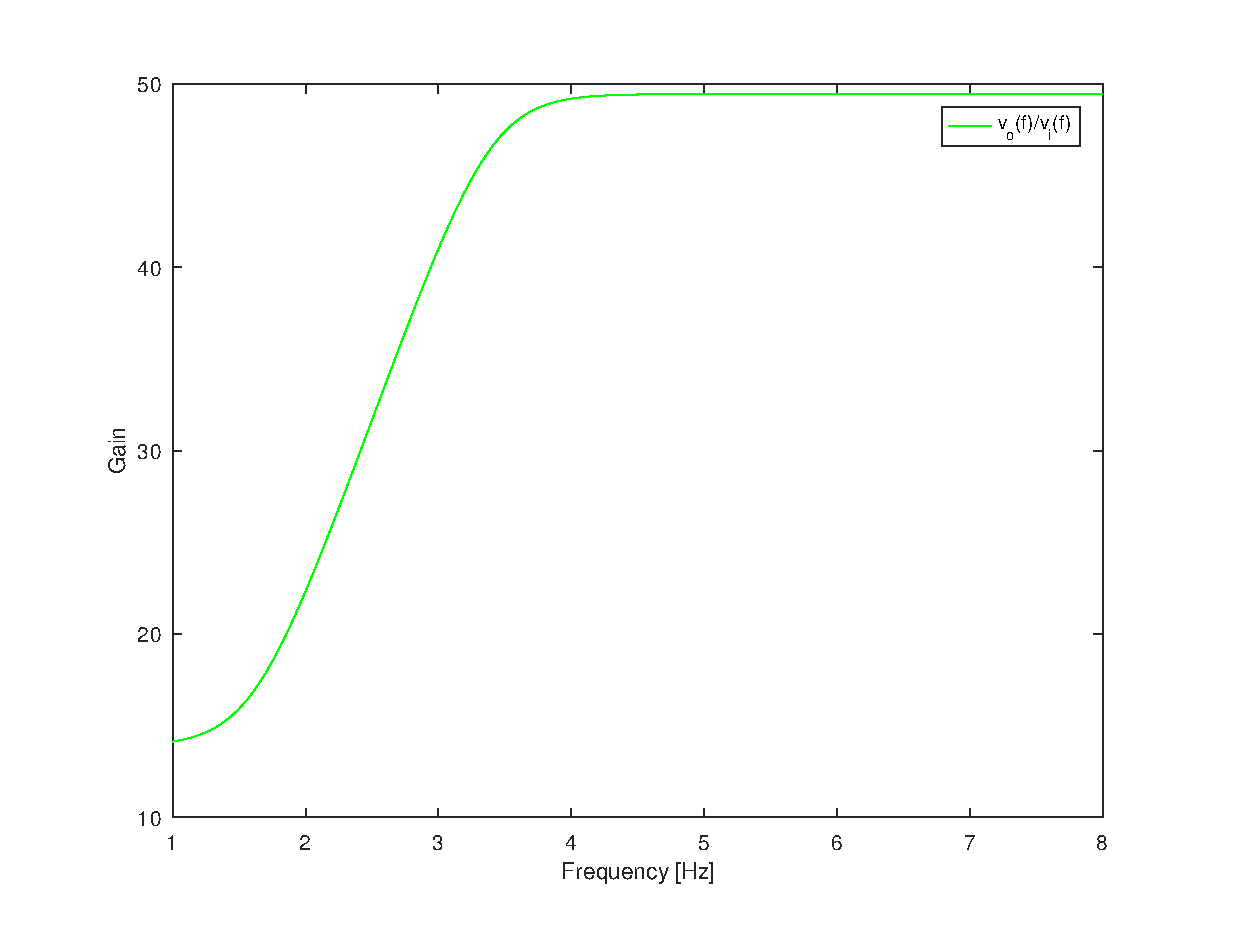
\includegraphics[width=.7\linewidth]{theo.eps}
  \caption{Gain [dB]. Octave}
  \label{fig:sim6} }
\parbox{.49\linewidth}{
  \centering
  \includegraphics[width=.65\linewidth]{gain.pdf}
  \caption{Gain [dB]. Ngspice}
  \label{fig:sim6}

}
\end{figure}



\begin{table}[ht]
\parbox{.45\linewidth}{
  \centering
  \begin{tabular}{|l|r|}
    \hline    
    {\bf Calculus} & {\bf Value [Ohm]} \\ \hline
    Zin & -738.418 + 125.718 j\\ \hline

  \end{tabular}
  \caption{Cirtcuit impedances. Variables are expressed in Ohm.(Ngspice)}} 
\parbox{.45\linewidth}{
 \centering
  \begin{tabular}{|l|r|}
    \hline    
    {\bf Name} & {\bf Value [Ohm]} \\ \hline
    \input{../mat/impedances_TAB}
  \end{tabular}
  \caption{Cirtcuit impedances. Variables are expressed in Ohm.(Octave)}}
\end{table}


We must also compare the phase plots. In octave, thanks to the capacitors we have 2 poles and 2 roots. However, in Ngspice we see 4 poles, again due to the complexity of the model used by this software.


\begin{figure}[ht]
\centering
\parbox{.49\linewidth}{
  \centering
  \includegraphics[width=.7\linewidth]{theo_phase.eps}
  \caption{Output voltage (phase). Octave}
  \label{fig:si} }
\parbox{.49\linewidth}{
  \centering
  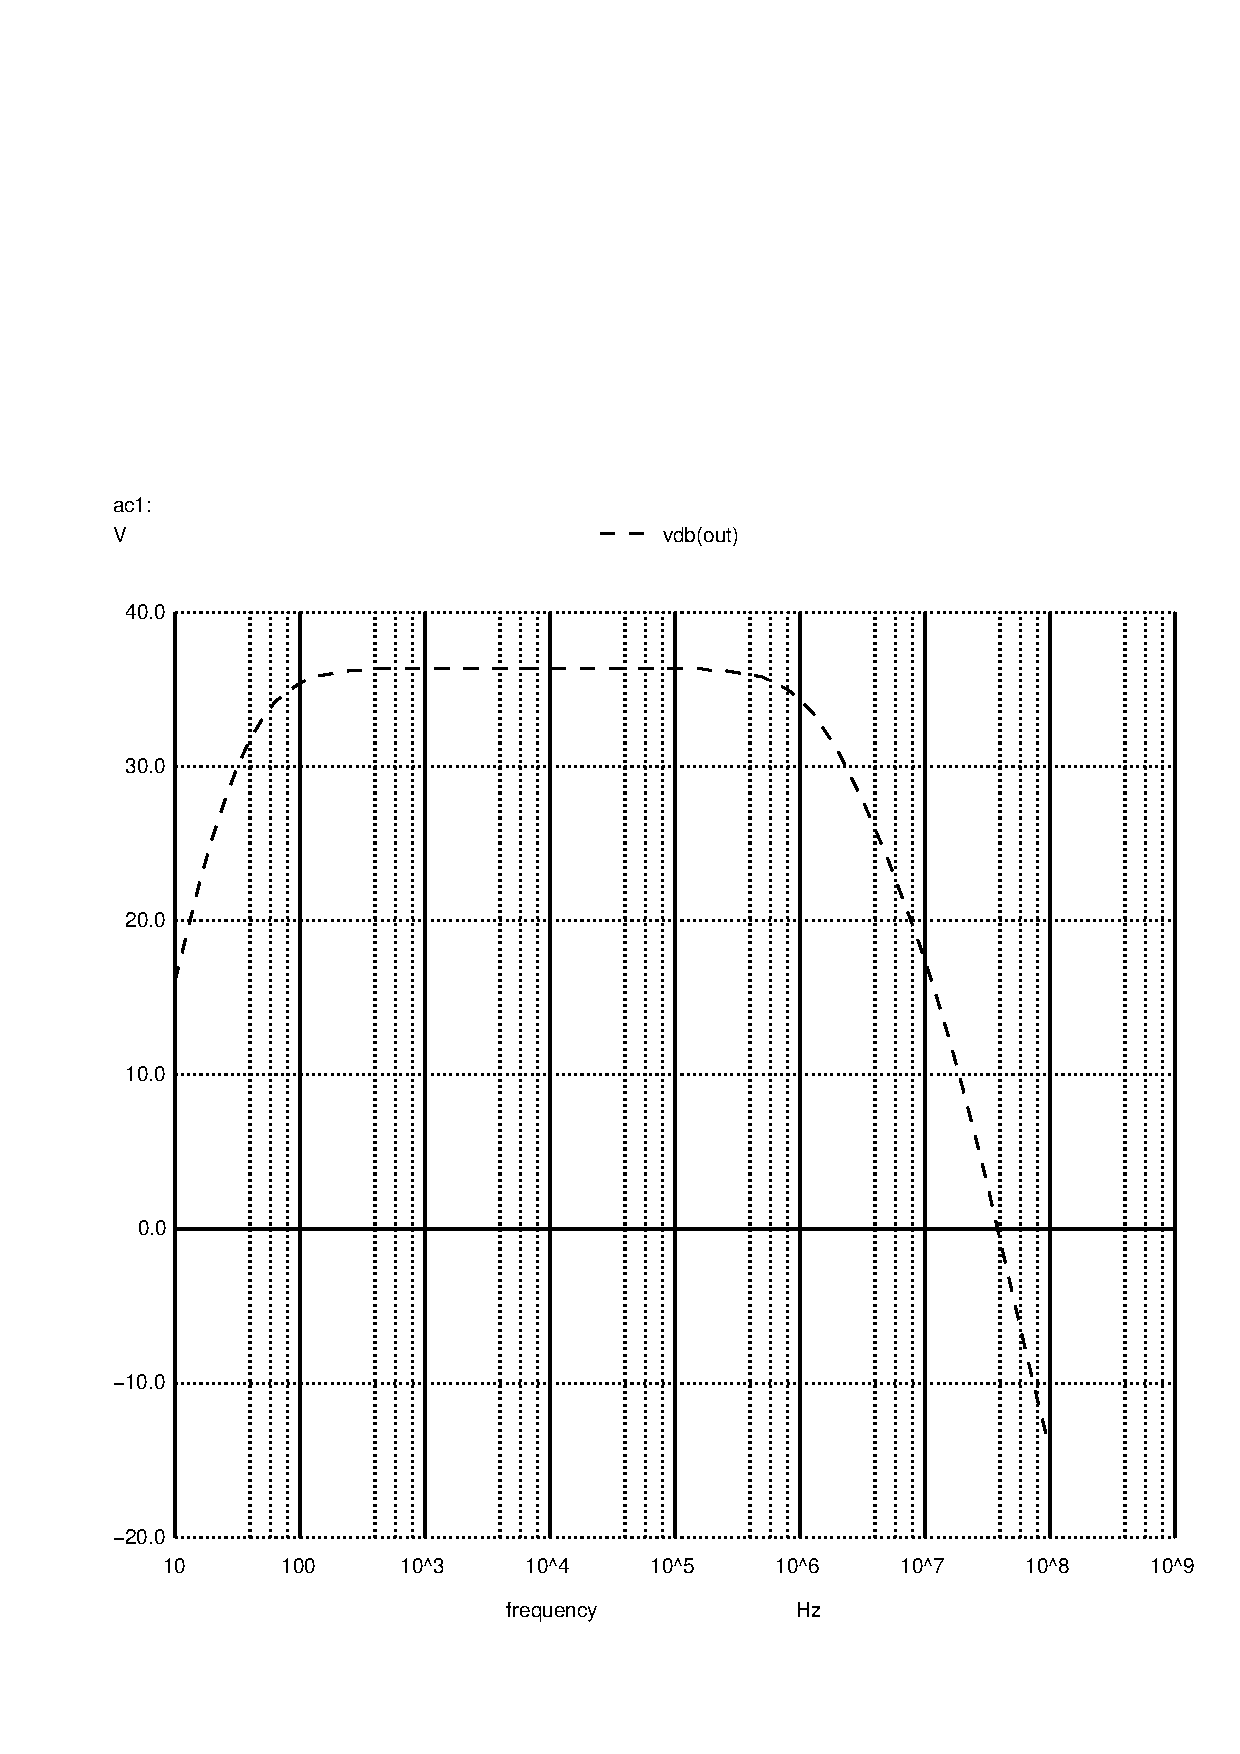
\includegraphics[width=.65\linewidth]{vo2f.pdf}
  \caption{Output voltage (phase). Ngspice}
  \label{fig:sim6}

}
\end{figure}




